% !TeX root = 02_intro_ml_polytech.tex
% !TeX encoding = UTF-8
% !TeX spellcheck = en_GB
\documentclass[t,10pt,aspectratio=169,rounded]{beamer}
\usetheme{CEA23}

\usepackage[utf8x]{inputenc}
\usepackage[english]{babel}
\usepackage{csquotes}
\usepackage{physics}
\usepackage{pgfplots}
\pgfplotsset{compat=1.18}

% Tikz styles
\usetikzlibrary{shadows, fit, backgrounds, positioning, shapes.geometric}
\tikzset{
  % Base style: rounded rectangle with a soft drop shadow
  set/.style = {
    rectangle,
    rounded corners = 8pt,
    draw = CEAblue,
    line width = 0.8pt,
    fill = CEAblue!5!white,
    inner sep = 12pt,
    drop shadow = {shadow xshift = 2pt, shadow yshift = -2pt,
                   opacity = 0.35, fill = black},
  },
  % Colour variants (inherit everything from `set`)
  set green/.style = {set, fill = CEAgreen!5!white, draw = CEAgreen},
  set red/.style   = {set, fill = CEAred!5!white,   draw = CEAred},
  % Label anchored at the upper-left corner, inside the set
  set label/.style = {
    anchor = south west,
    inner sep = 4pt,
    font = \bfseries\small,
  },
  % Element dot
  elem/.style = {circle, fill = black, inner sep = 1.2pt},
}

% Code listings: Carbon-style "code snapshot" cards (see code_listings_demo.tex)
\usepackage{beamer-code-listings}

\AtBeginSection[]{\sepframe[\insertsectionnumber]{}{}}

\begin{document}

\title{Introduction to Machine Learning}
\subtitle{Module 2 -- Machine Learning \\[0.5em] Practices, Optimisation, and Linear Models}
\date[02/12/2026]{2 December 2026}
\author{Riccardo \textsc{Finotello}}

\titlepagelogo{\includegraphics[height=24mm]{graphics/ORIGINAL/ISAS.png}}
\titlepagepicture{img/titlepage.png}
\setvalue{\diffusion}{}

\seminar[PolytechParis]{Machine Learning - PolytechParis}

\CEAmerci{See you next time!}
\CEAcenter{CEA SACLAY}
\addr{91\,191 Gif-sur-Yvette Cedex\\France}
\CEAemail{\href{mailto:riccardo.finotello@cea.fr}{\texttt{riccardo.finotello@cea.fr}}}

% --- TITLE SLIDE ---
\begin{frame}[plain]
  \titlepage
\end{frame}

% ------------------------------------------------------------------
% Content slides: drop your module slide fragments into 02_slides/
% and include them below, e.g.
%   \input{02_slides/section_01}
%   \input{02_slides/section_02}
% Each fragment contains \section{...} and \begin{frame}...\end{frame}
% only (no preamble, no \begin{document}).
% ------------------------------------------------------------------

% !TeX root = 02_intro_ml_polytech.tex
% !TeX encoding = UTF-8
% !TeX spellcheck = en_GB
\begin{frame}[fragile]{Welcome Back}{\includegraphics[height=12pt]{01_slides/img/tool.pdf}~What's in it for today?}

    Last time we got familiar with \textbf{Python} and manipulated the data we are going to use.
    You should all have saved two \texttt{.npy} files: one for the spectra, one for the annotations:
    \begin{enumerate}
        \item \alert<2>{\includegraphics[height=12pt]{01_slides/img/pen-tool.pdf}~Open the folder where you saved all your work}
        \item \alert<3>{\includegraphics[height=12pt]{01_slides/img/pen-tool.pdf}~Check that the \texttt{data} folder contains the two \texttt{.npy} files}
        \item \alert<4>{\includegraphics[height=12pt]{01_slides/img/pen-tool.pdf}~Launch the Jupyter notebook interface}
    \end{enumerate}

    \begin{onlyenv}<2>
        \begin{tikzpicture}[overlay]
            \node[yshift=-17em, xshift=-2em] at (current page.center) {
                \begin{codewithcard}{Terminal}
cd /path/to/your/folder
ls
                \end{codewithcard}
            };
        \end{tikzpicture}
    \end{onlyenv}

    \begin{onlyenv}<3>
        \begin{tikzpicture}[overlay]
    \node[label=right:data/, xshift=-2em, yshift=-10em] (data) at (current page.center) {\includegraphics[height=12pt]{01_slides/img/folder.pdf}};
    \node[below right=0.25em of data] (dots) {\dots};
    \node[below=0.25em of dots, label=right:HC\_labels.npy] (lab) {\includegraphics[height=12pt]{02_slides/img/numpy.pdf}};
    \node[below=0.25em of lab, label=right:HC\_norm.npy] (norm) {\includegraphics[height=12pt]{02_slides/img/numpy.pdf}};
    \node[below left=0.25em of norm, label=right:notebooks] (nb) {\includegraphics[height=12pt]{01_slides/img/folder.pdf}};
    \node[below=0.25em of nb, label=right:src] (src) {\includegraphics[height=12pt]{01_slides/img/folder.pdf}};
    \node[below=0.25em of src] (dots2) {\dots};

    \begin{scope}[on background layer]
        \node[set, fit=(data)(dots)(lab)(norm)(nb)(dots), minimum height=14em, minimum width=13em, xshift=4em, yshift=-2em] {};
    \end{scope}
\end{tikzpicture}

    \end{onlyenv}

    \begin{onlyenv}<4>
        \begin{tikzpicture}[overlay]
            \node[yshift=-17em, xshift=-2em] at (current page.center) {
                \begin{codewithcard}{Terminal}
uv run jupyter lab
                \end{codewithcard}
            };
        \end{tikzpicture}
    \end{onlyenv}

    \begin{onlyenv}<5>
        \vfill
        Today we will go through:
        \begin{itemize}
            \item ML practices: studying the data and \textbf{train/test splits}
            \item \textbf{Feature normalisation}: standardisation and other scaling techniques
            \item (Generalised) \textbf{Linear Models}: linear regression and logistic regression
            \item \textbf{Regularisation}: Lasso and Ridge regression
        \end{itemize}
    \end{onlyenv}
\end{frame}


\section{Machine Learning Best Practices}

\begin{frame}{Preparing a ML model}{The overfitting problem\dots}
    \begin{center}
        \def\overfitcurve{(0.30,1.10) (0.37,1.97) (0.45,1.90) (0.52,1.54) (0.59,1.25) (0.67,1.15) (0.74,1.25) (0.81,1.48) (0.89,1.77) (0.96,2.05) (1.03,2.25) (1.11,2.37) (1.18,2.38) (1.25,2.31) (1.33,2.18) (1.40,2.02) (1.47,1.86) (1.55,1.74) (1.62,1.67) (1.69,1.65) (1.77,1.69) (1.84,1.77) (1.92,1.86) (1.99,1.96) (2.06,2.04) (2.14,2.09) (2.21,2.09) (2.28,2.05) (2.36,1.98) (2.43,1.88) (2.50,1.78) (2.58,1.69) (2.65,1.62) (2.72,1.57) (2.80,1.52) (2.87,1.44) (2.94,1.33) (3.02,1.14) (3.09,0.92) (3.16,0.77) (3.20,0.80)}
\def\goodcurve{(0.30,1.05) (0.50,1.31) (0.70,1.54) (0.90,1.72) (1.10,1.87) (1.30,1.98) (1.50,2.04) (1.70,2.06) (1.90,2.05) (2.10,1.99) (2.30,1.88) (2.50,1.74) (2.70,1.55) (2.90,1.31) (3.10,1.03) (3.20,0.88)}
\def\underfitcurve{(0.30,1.69) (3.20,1.54)}
\def\trainpts{0.30/1.10, 0.62/1.19, 0.94/1.99, 1.27/2.29, 1.59/1.70,
    1.91/1.86, 2.23/2.08, 2.56/1.71, 2.88/1.43, 3.20/0.80}
\def\testpts{0.36/0.99, 0.98/1.68, 1.19/2.13, 2.10/2.21,
    2.52/1.85, 2.65/1.47, 2.80/1.53, 2.86/1.63}

\begin{tikzpicture}[
        train/.style={fill=CEAred, draw=none, circle, inner sep=1.6pt},
        test/.style={fill=CEAblue, draw=none, circle, inner sep=1.6pt},
        ax/.style={thick, CEAblack, ->}
    ]
    \foreach \xs/\firsttitle/\subtitle/\title/\curve/\col/\msetrain/\msetest/\name/\effect/\adjective in {
            0/Model 1/Overfitting/High Variance/\overfitcurve/CEAblack/0.0/0.153/overfitting/memorised the training data/unreliable,
            4.7/Model 2/Generalisation/Optimal/\goodcurve/CEAblack/0.044/0.030/generalisation/adjusted to the training data/great,
            9.4/Model 3/Underfitting/High Bias/\underfitcurve/CEAblack/0.200/0.148/underfitting/not learnt the training data/useless}
        {
            \begin{scope}[xshift=\xs cm]
                \draw[ax] (-0.2,0) -- (3.6,0) node[below] {$x$};
                \draw[ax] (0,-0.2) -- (0,3.0) node[left] {$y$};
                \node<1-3>[above] at (1.7,2.9) {\textbf{\firsttitle}};
                \node<4->[above] at (1.7,2.9) {\textcolor{CEAred}{\textbf{\title}}};
                \node<4->[above] at (1.7,3.4) {\footnotesize\textcolor{CEAred}{\textbf{\subtitle}}};
                \draw[\col, thick, smooth] plot coordinates {\curve};
                \foreach \px/\py in \trainpts \node[train] at (\px,\py) {};
                \only<3->{%
                \foreach \px/\py in \testpts \node[test] at (\px,\py) {};
                \node<2->[below, CEAred] at (1.7,-0.4) {$\operatorname{MSE}_{\text{train}}=\msetrain$};
                \node<3->[below, CEAblue] at (1.7,-0.9) {$\operatorname{MSE}_{\text{test}}=\msetest$};
                }

                \node<5->[below, CEAblack, align=center, text width=15em] at (1.7, -1.5) {\footnotesize The \textbf{\name} regime has \emph{\effect}. It is \textbf{\adjective} for new data.};
            \end{scope}
        }
\end{tikzpicture}

    \end{center}

    \vfill

    \begin{onlyenv}<1>
        \includesvg[height=12pt]{01_slides/img/brain.svg}~What would you consider as a \textbf{good model}? Think in terms of something like the \textbf{Mean Squared Error} (MSE):
        \begin{equation*}
            \operatorname{MSE}
            =
            \mathbb{E}\left[ \left( y - f(x) \right)^2 \right]
            =
            \mathbb{E}\left[ \operatorname{dist}\left( y - f(x) \right)^2 \right]
        \end{equation*}
    \end{onlyenv}

    \begin{onlyenv}<4>
        \begin{center}
            The model that seemed to work best, in reality \textbf{does not generalise}!
        \end{center}
    \end{onlyenv}

    \vfill
\end{frame}

\begin{frame}{Preparing a ML model}{How to avoid over- and under-fitting\dots}
    Suppose you have a \textbf{data distribution} $X = \left\{ x_i \right\}_{i = 1}^N$.
    Are there ways to avoid under- and overfitting?

    \begin{center}
        \begin{tikzpicture}
    \draw<1>[thick, draw=CEAred, fill=CEAred!5] (0, 0) rectangle (10cm, 1cm) node[midway] {DATA};
    \draw<2>[thick, draw=CEAred, fill=CEAred!5] (0, 0) rectangle (7cm, 1cm) node[midway] {TRAIN DATA};
    \draw<2>[thick, draw=CEAblue, fill=CEAblue!5] (7cm, 0) rectangle (10cm, 1cm) node[midway] {TEST DATA};
    \draw<3->[thick, draw=CEAred, fill=CEAred!5] (0, 0) rectangle (4cm, 1cm) node[midway] {TRAIN DATA};
    \draw<3->[thick, draw=CEAgreen, fill=CEAgreen!5] (4cm, 0) rectangle (7cm, 1cm) node[midway] {VALIDATION DATA};
    \draw<3->[thick, draw=CEAblue, fill=CEAblue!5] (7cm, 0) rectangle (10cm, 1cm) node[midway] {TEST DATA};
\end{tikzpicture}

    \end{center}

    \begin{itemize}[<+->]
        \item \textcolor{CEAred}{\textbf{Test Set:}} Split \textbf{randomly} your data to keep some of them for \textbf{testing}
        \item \textcolor{CEAred}{\textbf{Validation Set:}} Retain some more data to \textbf{validate} your choice of the ML model
        \item \textcolor{CEAred}{\textbf{Training Set:}} What remains is what you use to train the models (N.B. \alert{It must be representative of what you want to learn!})
    \end{itemize}

    \vfill \pause

    {\footnotesize
        \begin{tabular}{@{}llp{28em}@{}}
            \textbf{Glossary:} &                         &                                                                                                                                     \\
                               & \emph{testing:}         & It measures the \textbf{generalisation} capability of a ML model. \alert{Do not touch this data until you give your final results!} \\
                               & \emph{validation:}      & Scores the performance of the models on a distribution similar to that used in training                                             \\
                               & \emph{model selection:} & Choice of the \textbf{model} and \textbf{hyperparameters} that deliver the best results on validation                               \\
        \end{tabular}
    }
\end{frame}

\begin{frame}{Preparing a ML model}
    Let $\mathcal{D}$ be the whole data set.
    The procedure we just saw leaves you with:
    \begin{equation*}
        \mathcal{D} = \mathcal{D}_{\text{train}} \sqcup \mathcal{D}_{\text{val}} \sqcup \mathcal{D}_{\text{test}}
    \end{equation*}
    where
    \begin{enumerate}
        \item $x \in \mathcal{D}_{\text{test}}$ represent the real \textbf{use case} scenario
        \item $x \in \mathcal{D}_{\text{val}}$ come from the same distribution as $\mathcal{D}_{\text{train}}$ and are used for evaluation
        \item $x \in \mathcal{D}_{\text{train}}$ are \textbf{shuffled} data representing \textbf{realistic}
    \end{enumerate}
    This is known as \textbf{holdout validation}.

    \vfill

    {\footnotesize
        Once a \textbf{test set} is selected, there are other types of \textbf{validation} procedures worth knowing:
        \begin{itemize}
            \item \textbf{cross-validation}: Instead of choosing one validation set, you iteratively retain a certain number of data from the train distribution for validation and train on the others
            \item \textbf{leave-one-out} (\emph{jackknife}): Train on all but one piece of data and evaluate on the remaining point. Repeat for all samples at your disposal (extreme case of cross-validation).
        \end{itemize}
    }

    \vfill

    {\tiny Clearly, the more $\mathcal{D}_{\text{train}}$ \enquote{looks like} $\mathcal{D}_{\text{test}}$ the better!}
\end{frame}


\section{Optimisation and Loss Functions}

\begin{frame}{How do particles move?}{A little bit of physics\dots}
    \begin{columns}[c]
        \begin{column}{0.55\textwidth}
            Consider a \textbf{particle} (coords.\ $\vec{x}$) moving in a \textbf{potential}
            \begin{equation*}
                U(\vec{x})
            \end{equation*}

            \includegraphics[height=12pt]{01_slides/img/brain.pdf}~Where will it land when it reaches a \textbf{stable equilibrium}?
        \end{column}
        \hfil
        \begin{column}{0.4\textwidth}
            \def\points{(0.1, 2.0) (0.5, 1.4) (0.9, 1.2) (1.3, 1.5) (1.7, 1.8) (2.1, 1.7) (2.5, 0.6) (2.9, 0.65) (3.3, 1.1) (3.7, 1.2) (4.1, 0.3) (4.5, 0.6)}
\begin{tikzpicture}[
        ax/.style={thick, CEAblack, ->}
    ]
    \draw[ax] (-0.2,0) -- (5.0,0) node[below] {$\vec{x}$};
    \draw[ax] (0,-0.2) -- (0,3.0) node[left] {$U$};
    \draw[thick, CEAblack, smooth] plot coordinates {\points};

    \draw<1>[thick, CEAred, fill=CEAred!15] (1.9, 1.95) circle (0.1);
    \draw<2->[thick, CEAred, fill=CEAred!15] (4.15, 0.42) circle (0.1);
\end{tikzpicture}

        \end{column}
    \end{columns}

    \vfill

    \begin{onlyenv}<2->
        The \textbf{equilibrium} is reached when
        \begin{equation*}
            \vec{x}^{*} = \arg\min_{\vec{x} \in \mathbb{R}^d} U(\vec{x})
            \quad \Rightarrow \quad
            \vec{F} = \vec{\nabla} U(\vec{x}) = \vec{0},
        \end{equation*}
        which gives us a good criterion to find the \textbf{optimum}.
    \end{onlyenv}
\end{frame}

\begin{frame}{How do particles move?}{A little bit of physics\dots}
    \begin{columns}[c]
        \begin{column}{0.55\textwidth}
            So now suppose you have a set of \enquote{parameters} $\Theta = \{ \theta_i \}_{i = 1}^d$, governed by a function
            \begin{equation*}
                L = L(\Theta)
            \end{equation*}
        \end{column}
        \hfil
        \begin{column}{0.4\textwidth}
            %\begin{tikzpicture}[
        ax/.style={thick, ->, CEAblack},
        ellipse/.style={thick, dashed},
        path/.style={very thick, ->, CEAred}
    ]
    % Axes
    \draw[ax] (-0.25, 0.0) -- (4.0, 0.0) node[below] {$\theta_1$};
    \draw[ax] (0.0, -0.25) -- (0.0, 4.0) node[left] {$\theta_2$};

    % Profile
    \node (opt) at (2.0, 2.0) {};
    \draw[ellipse, CEAblue, fill=CEAblue!15, rotate around={34:(opt)}] (opt) ellipse (1.0 and 2.0);
    \draw[ellipse, CEAgreen, fill=CEAgreen!15, rotate around={34:(opt)}] (opt) ellipse (0.7 and 1.4);
    \draw[ellipse, CEAred, fill=CEAred!15, rotate around={34:(opt)}] (opt) ellipse (0.4 and 0.8);

    % Optimum
    \node<2->[star, star points=5, star point ratio=2.5, draw, fill=yellow] at (opt) {};

    % Path
    \draw<2->[path] (4.1, 3.2) -- (3.0, 2.6) -- (2.9, 1.8) -- (2.5, 1.5) -- (2.2, 1.9);
\end{tikzpicture}

        \end{column}
    \end{columns}
\end{frame}


\section{(Generalised) Linear Models}

% !TeX root = 02_intro_ml_polytech.tex
% !TeX encoding = UTF-8
% !TeX spellcheck = en_GB
\begin{frame}{Linear Regression}{Let's start simple\dots}
    Let $X \in \mathbb{R}^{N \times d}$ be our \textbf{data set} and $\vec{y} = \mathbb{R}^N$ be the labels:
    \begin{equation*}
        \mathcal{D} = \left\{ (\vec{x}_i, y_i) ~\mid~ \vec{x}_i \in \mathbb{R}^d,~ y_i \in \mathbb{R} \right\}_{i = 1}^N
    \end{equation*}

    \vfill \pause

    Consider a \textbf{Linear Regression} of $y$ using the data $X$:
    \begin{equation*}
        \vec{y} = X\, \vec{\beta}
    \end{equation*}

    \textbf{Objective:} find the \enquote{best} $\vec{\beta} = (\beta_1, \beta_2, \dots, \beta_d)$ to fit the data
\end{frame}

\begin{frame}{Linear Regression}{Defining the loss function\dots}
    The \textbf{loss function} encodes a \emph{distance} between predictions and true values:

    \vfill \pause

    \begin{block}{Mean Squared Error (L2/Gauss loss)}
        \begin{equation*}
            L\left(\vec{y}, \vec{y}^{(\Theta)}\right)
            =
            \frac{1}{2N} \sum\limits_{i = 1}^N \left(y_i - y^{(\Theta)}_i\right)^2
        \end{equation*}
    \end{block}

    \begin{onlyenv}<3>
        {\tiny
        \textcolor{CEAblack!65}{%
        Since $y_i^{(\Theta)} = \sum\limits_{\ell = 1}^d X_{i, \ell}\, \beta_{\ell}$, the L2 loss is the only case where the optimal values of $\vec{\beta}$ can be computed exactly:
        \begin{equation*}
            \pdv{L\left(y, y^{(\Theta)}\right)}{\beta_{\ell}}
            =
            \frac{1}{N} \sum\limits_{i = 1}^N X_{i\ell}\, \left(y_i - X_{i\ell}\, \beta_{\ell}\right)
            =
            0
            \quad \Leftrightarrow \quad
            \sum\limits_{i = 1}^N X_{i\ell} y_i
            =
            \beta_{\ell} \left( \sum\limits_{i = 1}^N X_{i\ell} X_{i\ell} \right)
            \quad \Leftrightarrow \quad
            X^{\top} \vec{y} = \left( X^{\top} X \right) \vec{\beta}
        \end{equation*}
        which means that the coefficients are:
        \begin{equation*}
            \vec{\beta}
            =
            \left( X^{\top} X \right)^{-1} X^{\top} \vec{y}.
        \end{equation*}
        In other words, no need for gradient descent, here.
        }
        }
    \end{onlyenv}
\end{frame}

\begin{frame}{Linear Regression}{Defining the loss function\dots}
    \begin{block}{Mean Absolute Error (L1/Laplace loss)}
        \begin{equation*}
            L\left(\vec{y}, \vec{y}^{(\Theta)}\right)
            =
            \frac{1}{N} \sum\limits_{i = 1}^N \left|y_i - y^{(\Theta)}_i\right|
        \end{equation*}
    \end{block}

    \begin{block}{Mean Squared Percentage Error}
        \begin{equation*}
            L\left(\vec{y}, \vec{y}^{(\Theta)}\right)
            =
            \frac{1}{2N} \sum\limits_{i = 1}^N \left( \frac{y_i - y^{(\Theta)}_i}{y_i} \right)^2
        \end{equation*}
    \end{block}

    \begin{block}{Huber Loss}
        \small
        \begin{equation*}
            L\left(\vec{y}, \vec{y}^{(\Theta)}\right)
            =
            \frac{1}{2N} \sum\limits_{i = 1}^N \left(y_i - y^{(\Theta)}_i\right)^2\, \Theta\left( \delta - \left|y_i - y^{(\Theta)}_i\right|\right)
            +
            \frac{1}{N} \sum\limits_{i = 1}^N \left|y_i - y^{(\Theta)}_i\right|\, \Theta\left( \left|y_i - y^{(\Theta)}_i\right| - \delta \right)
        \end{equation*}
    \end{block}
\end{frame}

\begin{frame}{Constrained Optimisation}{Regularizing your models\dots}
    We saw that finding the \textbf{optimum} $\simeq$ finding equilibrium (\enquote{$\vec{F} = \vec{\nabla} L = 0$}).

    \vfill \pause

    What if we wanted to find the \textbf{optimum} in a particular situation?
    For instance:
    \begin{center}
        \emph{%
            Find the optimum of $L(\theta_1, \theta_2) = \theta_1^2 + \theta_2^2$ such that $g(\theta_1, \theta_2) = \theta_1 + \theta_2 - 1 = 0$?
        }
    \end{center}

    \vfill

    \begin{center}
        \includegraphics[height=0.4\textheight]{02_slides/img/intersecting_plane.png}
        \hfil
        \includegraphics[height=0.4\textheight]{02_slides/img/intersecting_plane_2.png}
    \end{center}
\end{frame}

\begin{frame}{Constrained Optimisation}{\includegraphics[height=12pt]{01_slides/img/tool.pdf}~Equality constraints}
    We use \textbf{Lagrange multipliers} and promote:
    \begin{equation*}
        L(\theta_1, \theta_2)
        \quad \rightarrow \quad
        \tilde{L}(\theta_1, \theta_2, \lambda)
        =
        L(\theta_1, \theta_2) + \lambda\, g(\theta_1, \theta_2)
    \end{equation*}

    \vfill \pause

    When we compute the gradient of $\tilde{L}$, we now have:
    \begin{enumerate}
        \item $\pdv{\tilde{L}}{\theta_1} = 0$ and $\pdv{\tilde{L}}{\theta_2} = 0$: these are the \enquote{old} equations (nothing changed)
        \item $\pdv{\tilde{L}}{\lambda} = 0 \Leftrightarrow g(\theta_1, \theta_2) = 0$: this condition automatically imposes the constraint!
    \end{enumerate}

    \vfill \pause

    \includegraphics[height=12pt]{01_slides/img/pen-tool.pdf}~Solve the problem from the previous slide (\emph{pen and paper})!

    \vfill \pause

    \textcolor{CEAblack!65}{%
        \begin{equation*}
            \begin{cases}
                \pdv{\tilde{L}(\theta_1, \theta_2, \lambda)}{\theta_1} & = 2 \theta_1 + \lambda = 0    \\
                \pdv{\tilde{L}(\theta_1, \theta_2, \lambda)}{\theta_2} & = 2 \theta_2 + \lambda = 0    \\
                \pdv{\tilde{L}(\theta_1, \theta_2, \lambda)}{\lambda}  & = \theta_1 + \theta_2 - 1 = 0 \\
            \end{cases}
            \Leftrightarrow
            \begin{cases}
                \theta_1 - \theta_2  & = 0 \\
                \lambda + 2 \theta_2 & = 0 \\
                \theta_1 + \theta_2  & = 1 \\
            \end{cases}
            \Leftrightarrow
            \begin{cases}
                \theta_1 & = \frac{1}{2} \\
                \theta_2 & = \frac{1}{2} \\
                \lambda  & = - 1         \\
            \end{cases}
            \Rightarrow
            L(\theta_1, \theta_2) = \frac{1}{2}.
        \end{equation*}
    }
\end{frame}

\begin{frame}{Constrained Optimisation}{What about milder constraints?}
    \begin{center}
        \emph{%
            Find the optimum of $L(\theta_1, \theta_2) = \theta_1^2 + \theta_2^2$ such that $g(\theta_1, \theta_2) = 4 - \theta_1^2 - \theta_2^2 \le 0$
        }

        {\tiny Find the minimum, but \enquote{above} the circle $\theta_1^2 + \theta_2^2 = 4$}
    \end{center}

    \vfill \pause

    We can proceed as before:
    \begin{equation*}
        \tilde{L}(\theta_1, \theta_2, \lambda)
        =
        L(\theta_1, \theta_2) + \lambda\, g(\theta_1, \theta_2)
        \alert{\quad \text{such that} \quad \lambda \ge 0}
    \end{equation*}
    and realise that
    \begin{columns}[c]
        \begin{column}{0.6\textwidth}
            \only<2>{%
                \begin{equation*}
                    (\theta_1^*, \theta_2^*, \lambda^*)
                    =
                    \arg\min\limits_{\theta_1, \theta_2}
                    \begin{cases}
                        L(\theta_1, \theta_2) & \qif g(\theta_1, \theta_2) \le 0
                        \\
                        \infty                & \qif g(\theta_1, \theta_2) > 0
                    \end{cases}
                \end{equation*}
            }
            \only<3->{%
            \begin{equation*}
                (\theta_1^*, \theta_2^*, \lambda^*)
                =
                \underbrace{%
                    \arg\min\limits_{\theta_1, \theta_2}
                    \arg\max\limits_{\lambda}
                    \tilde{L}(\theta_1, \theta_2, \lambda)
                }_{\text{saddle point!}}
            \end{equation*}
            and
            \begin{equation*}
                \lambda^*\, g(\theta_1^*, \theta_2^*) = 0
            \end{equation*}

            {\tiny Either the \alert<4>{constraint is active} and $\lambda > 0$, or the \alert<5>{constraint is satisfied} and $\lambda = 0$}
            }
        \end{column}
        \hfil
        \begin{column}{0.35\textwidth}
            \centering
            \begin{tikzpicture}
    % Axes
    \draw[thick, ->] (-0.25, 0.0) -- (3.0, 0.0) node[below] {$\theta_1$};
    \draw[thick, ->] (0.0, -0.25) -- (0.0, 3.0) node[left] {$\theta_2$};

    % Ellipses
    \draw[thin, CEAblue, fill=CEAblue!25] (1.5, 1.5) ellipse (0.75 and 1.25);
    \draw[thin, CEAgreen, fill=CEAgreen!25] (1.5, 1.5) ellipse (0.5 and 0.75);
    \draw[thin, CEAred, fill=CEAred!25] (1.5, 1.5) ellipse (0.25 and 0.25);

    % Avoid area
    \draw<3->[thin, CEAblack, fill=CEAblack!85] (1.5, 1.5) node[white] {$\infty$} circle (0.65);

    % Possible minima
    \draw<4>[CEAred, fill=CEAred!50] (1.5, 1.65) circle (2pt);
    \draw<4>[CEAred, fill=CEAred] (1.5, 2.15) circle (2pt);
    \draw<4>[CEAred, dashed, ->] (1.5, 1.70) -- (1.5, 2.05);

    \draw<5>[CEAred, fill=CEAred] (1.75, 2.5) circle (2pt);
\end{tikzpicture}

        \end{column}
    \end{columns}
\end{frame}

\begin{frame}{Constrained Optimisation}{\includegraphics[height=12pt]{01_slides/img/tool.pdf}~Inequality constraints}
    \includegraphics[height=12pt]{01_slides/img/pen-tool.pdf}~Solve the problem from the previous slide (\emph{pen and paper})!

    \vfill \pause

    \textcolor{CEAblack!65}{%
        In this scenario, the constraint is active:
        \begin{equation*}
            \footnotesize
            \begin{cases}
                \pdv{\tilde{L}(\theta_1, \theta_2, \lambda)}{\theta_1} = 2 (1 - \lambda) \theta_1 & = 0   \\
                \pdv{\tilde{L}(\theta_1, \theta_2, \lambda)}{\theta_2} = 2 (1 - \lambda) \theta_2 & = 0   \\
                4 - \theta_1^2 - \theta_2^2                                                       & \le 0 \\
                \lambda^* (4 - \theta_1^{*\, 2} - \theta_2^{*\, 2})                               & = 0
            \end{cases}
            \quad \Leftrightarrow \quad
            \begin{cases}
                \lambda^*                           & = 1                \\
                \theta_1^{*\, 2} + \theta_2^{*\, 2} & = 4                \\
                \theta_1                            & = u \in \mathbb{R} \\
                \theta_2                            & = v \in \mathbb{R}
            \end{cases}
        \end{equation*}
    }
    \begin{center}
        \begin{tikzpicture}[scale=0.6, every node/.style={scale=0.6}]
    % Values
    \draw[CEAblue, fill=CEAblue!25] (0, 0) circle (2.0);
    \draw[CEAgreen, fill=CEAgreen!25] (0, 0) circle (1.25);
    \draw[CEAred, fill=CEAred!25] (0, 0) circle (0.5);

    % Axes
    \draw[thick, CEAblack, ->] (-2.5, 0.0) -- (2.5, 0.0) node[below] {$\theta_1$};
    \draw[thick, CEAblack, ->] (0.0, -2.5) -- (0.0, 2.5) node[left] {$\theta_2$};

    % Avoid
    \draw<3->[CEAblack, fill=CEAblack!85] (0, 0) circle (0.75);
    \node<3->[CEAblack, anchor=west] at (0.4, 0.7) {$\theta_1^2 + \theta_2^2 = 4$};

    % Optima
    \draw<4->[CEAred, ultra thick, fill=none] (0, 0) circle (0.75);
\end{tikzpicture}

    \end{center}
\end{frame}

\begin{frame}{Avoid Overfitting}{Constraints as solution to your problems\dots}
    How does all this help us?

    \vfill \pause

    \includegraphics[height=12pt]{01_slides/img/brain.pdf}~Do you remember the \textbf{overfitting problem}?

    \vfill \pause

    We can avoid (partially) overfitting by constraining the parameters:
    \begin{equation*}
        L\left(\vec{y}, \vec{y}^{(\Theta)}\right)
        =
        \underbrace{\operatorname{MSE}\left(\vec{y}, \vec{y}^{(\Theta)}\right)}_{\text{\enquote{standard} loss}}
        \only<4,6->{+ \alpha\, \sum\limits_{i = 1}^d \theta_i^2}
        \only<5,6->{+ \beta\, \sum\limits_{i = 1}^d \left| \theta_i \right|}
    \end{equation*}
    \begin{itemize}
        \item<4,6-> $\sum\limits_{i = 1}^d \theta_i^2 \le \epsilon$: this is called \textbf{ridge regression} (or \emph{L2 regularisation})
        \item<5,6-> $\sum\limits_{i = 1}^d \abs{\theta_i} \le \epsilon$: this is called \textbf{lasso regression} (or \emph{L1 regularisation})
        \item<6-> both of them at the same time: this is called \textbf{elastic net} regression
    \end{itemize}
    {\footnotesize
    The idea is to avoid the \enquote{explosion} of the parameters and exploit them when they are \enquote{small}.
    }
\end{frame}

\begin{frame}{Avoid Overfitting}{How to evaluate your models?}
    Suppose we have \enquote{true values} $\vec{y}$ and \textbf{predictions} $\vec{y}^{(\Theta)}$.
    How to measure \textbf{how good} the model is?

    \vfill \pause

    \textbf{Coefficient of Determination:} (\emph{R-squared})
    \begin{equation*}
        R^2 = 1 - \frac{\sum\limits_{i = 1}^d (y_i - y_i^{(\Theta)})^2}{\sum\limits_{i = 1}^d (y_i - \mathbb{E}[y_i^{(\Theta)}])^2}
    \end{equation*}
    and others that you already know (mean squared error, mean absolute error, percentage errors, etc.).
    Take a look at \href{https://scikit-learn.org/stable/api/sklearn.metrics.html\#regression-metrics}{Scikit-learn regression metrics} for a nice list!

    \vfill \pause

    \textbf{N.B.:} Metrics computed on the training set give only a rough idea of how the model is able to fit some data.
    Only \textbf{test metrics} must be used to score the ability of the model to generalise!
\end{frame}

\begin{frame}[fragile]{Avoid Overfitting}{\includegraphics[height=12pt]{01_slides/img/tool.pdf}~Some hands-on on regression\dots}
    \begin{enumerate}
        \item \alert<2>{\includegraphics[height=12pt]{01_slides/img/pen-tool.pdf}~Create a new notebook \texttt{linear\_models.ipynb}}
        \item \alert<3>{\includegraphics[height=12pt]{01_slides/img/pen-tool.pdf}~Import the \texttt{api} module of the library \texttt{statsmodels} as \texttt{sm}}
        \item \alert<4>{\includegraphics[height=12pt]{01_slides/img/pen-tool.pdf}~Generate some random data using \texttt{numpy}}
        \item \alert<5>{\includegraphics[height=12pt]{01_slides/img/pen-tool.pdf}~Create an arbitrary \textbf{linear model} using your data and some parameters of your choice (remember to also add a column to the data for the intercept!)}
        \item \alert<6>{\includegraphics[height=12pt]{01_slides/img/pen-tool.pdf}~Split the data in training and test sets}
        \item \alert<7>{\includegraphics[height=12pt]{01_slides/img/pen-tool.pdf}~Define the \textbf{Ordinary Least Squares} model (linear model) using \texttt{sm.OLS}}
        \item \alert<8>{\includegraphics[height=12pt]{01_slides/img/pen-tool.pdf}~Fit the OLS to your data and print the summary of the results.}
        \item \alert<9>{\includegraphics[height=12pt]{01_slides/img/pen-tool.pdf}~Compute the predictions and their coefficient of determination ($R^2$)}
        \item \alert<10>{\includegraphics[height=12pt]{01_slides/img/pen-tool.pdf}~Fit a L1-regularised model and a L2-regularised model and compare the performance}
    \end{enumerate}

    \begin{onlyenv}<3>
        \begin{tikzpicture}[overlay]
            \node[set, yshift=-2em, xshift=-2em] at (current page.center) {
                \begin{notebookin}
import statsmodels.api as sm
                \end{notebookin}
            };
        \end{tikzpicture}
    \end{onlyenv}

    \begin{onlyenv}<4>
        \begin{tikzpicture}[overlay]
            \node[set, yshift=-2em, xshift=-2em] at (current page.center) {
                \begin{notebookin}
import numpy as np
X = np.random.randn(1000, 3)
                \end{notebookin}
            };
        \end{tikzpicture}
    \end{onlyenv}

    \begin{onlyenv}<5>
        \begin{tikzpicture}[overlay]
            \node[set, yshift=1em, xshift=-2em] at (current page.center) {
                \begin{notebookin}
X = sm.add_constant(X)  # or np.concat([np.ones((1000,1)), X], axis=1)
theta = np.array([-0.12, 0.05, 0.3, -0.05])
y = X @ theta + 0.5 * np.random.randn(1000)
                \end{notebookin}
            };
        \end{tikzpicture}
    \end{onlyenv}

    \begin{onlyenv}<6>
        \begin{tikzpicture}[overlay]
            \node[set, yshift=1em, xshift=-2em] at (current page.center) {
                \begin{notebookin}
X_train = X[:750]; y_train = y[:750]
X_test = X[750:]; y_test = y[750:]
                \end{notebookin}
            };
        \end{tikzpicture}
    \end{onlyenv}

    \begin{onlyenv}<7>
        \begin{tikzpicture}[overlay]
            \node[set, yshift=-2em, xshift=-2em] at (current page.center) {
                \begin{notebookin}
ols = sm.OLS(y_train, X_train)
                \end{notebookin}
            };
        \end{tikzpicture}
    \end{onlyenv}

    \begin{onlyenv}<8>
        \begin{tikzpicture}[overlay]
            \node[set, text width=30em, yshift=-4em, xshift=-2em] at (current page.center) {
                \begin{notebookin}
results = ols.fit()
print(results.summary())
                \end{notebookin}
                \includegraphics[height=0.5\textheight]{02_slides/img/summary_ols.png}
            };
        \end{tikzpicture}
    \end{onlyenv}

    \begin{onlyenv}<9>
        \begin{tikzpicture}[overlay]
            \node[set, text width=30em, yshift=-4em, xshift=-2em] at (current page.center) {
                \begin{notebookin}
from sklearn.metrics import r2_score

preds = results.predict(X_test)
r2 = r2_score(y_test, preds)
print("R-squared =", r2)
                \end{notebookin}
                \begin{notebookout}
R-squared = 0.10428474173501134
                \end{notebookout}
            };
        \end{tikzpicture}
    \end{onlyenv}

    \begin{onlyenv}<10>
        \begin{tikzpicture}[overlay]
            \node[set, text width=30em, yshift=-4em, xshift=-2em] at (current page.center) {
                \begin{notebookin}
results_l1 = ols.fit_regularized(alpha=0.05, L1_wt=1.0)
preds_l1 = results_l1.predict(X_test)
r2_l1 = r2_score(y_test, preds_l1)
results_l2 = ols.fit_regularized(alpha=0.1, L1_wt=0.0)
preds_l2 = results_l2.predict(X_test)
r2_l2 = r2_score(y_test, preds_l2)
print("R-squared (L1) =", r2_l1)
print("R-squared (L2) =", r2_l2)
                \end{notebookin}
                \begin{notebookout}
R-squared (L1) = 0.11323501063060759
R-squared (L2) = 0.12657738085806358
                \end{notebookout}
            };
        \end{tikzpicture}
    \end{onlyenv}
\end{frame}

\begin{frame}{Linear Models for Classification}{From regression to classification\dots}
    For now we worked with
    \begin{equation*}
        \vec{x} \in \mathbb{R}^{d}
        \quad \text{and} \quad
        y \in \mathbb{R}
    \end{equation*}

    But what if $y$ is \textbf{categorical}? Such as
    \begin{equation*}
        y \in \{ \text{cat}, \text{dog}, \text{elephant}, \dots \}
    \end{equation*}

    \vfill \pause

    This can happen for both \textbf{data} and \textbf{labels} and the only way is to convert it to numerical:
    \begin{equation*}
        \{ \text{cat}, \text{dog}, \text{elephant}, \dots \} \mapsto \{ 0, 1, 2, \dots \}
    \end{equation*}
    which establishes to which \textbf{class} a particular piece of data belongs.
\end{frame}

\begin{frame}{Linear Models for Classification}{From regression to classification\dots}
    What information do we get from \textbf{class} assignments?

    \vfill \pause

    \begin{center}
        Does $\vec{x}_i$ belong to class 1? Does $\vec{x}_i$ belong to class 2? etc.
    \end{center}

    \vfill \pause

    You can think of them in terms of their \textbf{one-hot encoding}:
    \begin{center}
        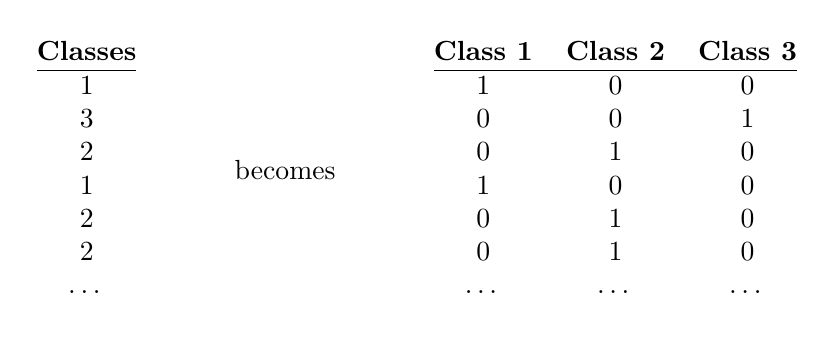
\begin{tikzpicture}
            \node (classes) at (0, 0) {
                \begin{tabular}{@{}c@{}}
                    \textbf{Classes} \\ \hline
                    1                \\
                    3                \\
                    2                \\
                    1                \\
                    2                \\
                    2                \\
                    \dots
                \end{tabular}
            };
            \node[right=of classes] (middle) {becomes};
            \node[right=of middle] (oh) {
                \begin{tabular}{@{}ccc@{}}
                    \textbf{Class 1} & \textbf{Class 2} & \textbf{Class 3} \\ \hline
                    1                & 0                & 0                \\
                    0                & 0                & 1                \\
                    0                & 1                & 0                \\
                    1                & 0                & 0                \\
                    0                & 1                & 0                \\
                    0                & 1                & 0                \\
                    \dots            & \dots            & \dots
                \end{tabular}
            };
        \end{tikzpicture}
    \end{center}
\end{frame}

\begin{frame}{Linear Models for Classification}{From regression to classification\dots}
    That is, with $K$ different classes
    \begin{equation*}
        \operatorname{OH}_K(y)
        =
        \begin{cases}
            1 & \qif y = k    \\
            0 & \qif y \neq k
        \end{cases}
    \end{equation*}

    \vfill \pause

    This allows us to answer
    \begin{center}
        With what probability does the \textbf{event} $\vec{x}$ belong to class $y$?
    \end{center}
    \begin{equation*}
        P(y = k \mid \vec{x})
    \end{equation*}
    {\tiny Remember the Naive Bayes Classifier of the first day?}

    \vfill \pause

    How to create a \textbf{predictive model} for $P(y = k \mid \vec{x})$?
\end{frame}

\begin{frame}{Linear Models for Classification}{Log-odds and linear models\dots}
    Let's call the \textbf{predicted probability} that an event is in class $k$ using a \textbf{model} with parameters $\Theta$:
    \begin{equation*}
        y_k^{(\Theta)} = P(y = k \mid \vec{x}, \Theta) \in [0, 1]
    \end{equation*}

    What are the \textbf{odds} that this is true?
    \begin{equation*}
        \text{logit}_k
        =
        \ln \underbrace{\frac{y_k^{(\Theta)}}{1 - y_k^{(\Theta)}}}_{\text{odds}}
        =
        \frac{\text{\enquote{This happens}}}{\text{\enquote{This does not happen}}}
        \in (-\infty, +\infty)
    \end{equation*}

    \vfill

    \includegraphics[height=12pt]{01_slides/img/brain.pdf}~What are the odds that an \textbf{unbiased} coin gives either head or tail?

    \includegraphics[height=12pt]{01_slides/img/brain.pdf}~What are the odds that an \textbf{biased} (80\% head) coin gives either head or tail?
\end{frame}

\begin{frame}{Linear Models for Classification}{Log-odds and linear models\dots}
    What is the simplest next step to define a model?
    Consider the model
    \begin{equation*}
        \text{logit}_k = f_{k, (\Theta)}(\vec{x}) = \sum\limits_{f = 1}^d x_f \underbrace{\Theta_{f\, k}}_{\text{matrix!}}
    \end{equation*}
    and let $f_{k,\, (\Theta)}$ be a \textbf{linear model}:
    \begin{equation*}
        \ln \frac{y_k^{(\Theta)}}{1 - y_k^{(\Theta)}}
        =
        f_{k,\, (\Theta)}(\vec{x})
        =
        \theta_{1k}\, x_1
        +
        \theta_{1k}\, x_2
        +
        \dots
    \end{equation*}
    This is called
    \begin{center}
        \textbf{Generalised Linear Model}
    \end{center}
    {\tiny You are not fitting a linear model on $y$, but on the log-odds, hence the \enquote{generalised}}
\end{frame}

\begin{frame}{Linear Models for Classification}{\includegraphics[height=12pt]{01_slides/img/tool.pdf}~Log-odds and linear models\dots}
    The peculiarity of the model is that $y_{(\Theta)}$ has a particular shape:

    \vfill

    \includegraphics[height=12pt]{01_slides/img/pen-tool.pdf}~Solve the previous equation for $y_{(\Theta)}$

    \vfill \pause

    \begin{columns}[c]
        \begin{column}{0.5\textwidth}
            The predictions follow a \textbf{logistic} curve (\emph{sigmoid}):
            \begin{equation*}
                y_k^{(\Theta)}
                =
                P(y = k \mid \vec{x})
                =
                \frac{1}{1 + e^{-f_{k,\, (\Theta)}(\vec{x})}}
                \in [0, 1]
            \end{equation*}
            which enables \textbf{class assignments}:
            \begin{equation*}
                \hat{y}^{(\Theta)} = k \qif y_k^{(\Theta)} > t
            \end{equation*}
            where $t \in [0, 1]$ is a choice.
        \end{column}
        \begin{column}{0.5\textwidth}
            \centering
            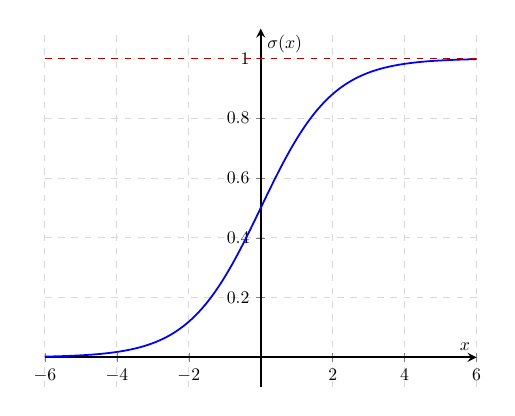
\begin{tikzpicture}[scale=0.8, every node/.style={scale=0.8}]
    \begin{axis}[
            axis lines = middle,
            xlabel = {$x$},
            ylabel = {$\sigma(x)$},
            xmin = -6, xmax = 6,
            ymin = -0.1, ymax = 1.1,
            domain = -6:6,
            samples = 100,
            smooth,
            thick,
            grid = major,
            grid style = {dashed, gray!30},
            legend pos = north west
        ]
        % Standard Logistic (Sigmoid) Function: f(x) = 1 / (1 + exp(-x))
        \addplot[color=blue] {1 / (1 + exp(-x))};

        % Asymptotic Boundaries y = 0 and y = 1
        \draw[dashed, red!70!black, thin] (axis cs:-6,1) -- (axis cs:6,1);

    \end{axis}
\end{tikzpicture}

        \end{column}
    \end{columns}
\end{frame}

\begin{frame}{Linear Models for Classification}{Multi-class classification and linear models\dots}
    What if classes are \textbf{not independent} (i.e.\ $\vec{x}$ can be $A$ or $B$, but not both)?

    \vfill

    In this case, we must also impose that the \textbf{sum of all probabilities} is 1:
    \begin{equation*}
        \sum\limits_{k = 1}^K P(y = k \mid \vec{x}) = 1
    \end{equation*}
    Hence, we get:
    \begin{equation*}
        y_k^{(\Theta)}
        =
        \frac{e^{f_{k,\, (\Theta)}(\vec{x})}}{\sum\limits_{h = 1}^K e^{f_{h,\, (\Theta)}(\vec{x})}}
        =
        \operatorname{softmax}(f_{k,\, (\Theta)}(\vec{x}))
    \end{equation*}

    \vfill \pause

    \begin{center}
        How to train a classification model?

        {\tiny \textbf{Spoiler:} it is not as simple as just comparing \enquote{errors}}
    \end{center}
\end{frame}

\begin{frame}{Linear Models for Classification}{Comparing distributions\dots}
    Suppose you have a system of particles $x \in \mathcal{X}$:
    \begin{center}
        \begin{tikzpicture}[scale=0.75, every node/.style={scale=0.75}]
    \draw[ultra thick, CEAblack] (0, 0) -- (3, 0) -- (3, 3) -- (0, 3) --cycle;

    \draw[CEAred, fill=CEAred!50] (1.0, 0.5) circle (3pt);
    \draw[CEAred, fill=CEAred!50] (1.0, 1.5) circle (3pt);
    \draw[CEAred, fill=CEAred!50] (2.0, 1.5) circle (3pt);
    \draw[CEAred, fill=CEAred!50] (2.5, 2.5) circle (3pt);
    \draw[CEAred, fill=CEAred!50] (0.5, 2.15) circle (3pt);
    \draw[CEAred, fill=CEAred!50] (0.75, 1.45) circle (3pt);
    \draw[CEAred, fill=CEAred!50] (1.75, 1.35) circle (3pt);
    \draw[CEAred, fill=CEAred!50] (0.9, 1.65) circle (3pt);
    \draw[CEAred, fill=CEAred!50] (1.2, 1.25) circle (3pt);
\end{tikzpicture}

    \end{center}
    and you want to study its distribution (its \emph{disorder}).
    You measure its entropy:
    \begin{equation*}
        H(P) = - \sum\limits_{x \in \mathcal{X}} P(x) \ln P(x) = - \mathbb{E}_P[\ln P]
    \end{equation*}

    \vfill

    And if more systems become available, you then \textbf{sum} the entropies:
    \begin{equation*}
        H_{\text{tot}}(P)
        =
        H_1(P) + H_2(P) + \dots
    \end{equation*}
\end{frame}

\begin{frame}{Linear Models for Classification}{Comparing distributions\dots}
    In this case, we have \textbf{two distributions} for \textbf{each class} (system):
    \begin{enumerate}
        \item the \textbf{true labels} $y_k \sim P$: the \textbf{one-hot} values of the labels in the data set
        \item the \textbf{predicted labels} $y_k^{(\Theta)} \sim Q$: the probabilities of belonging to class $k$
    \end{enumerate}

    \vfill

    To compare them, we use the \textbf{cross-entropy} as \textbf{loss function}:
    \begin{equation*}
        H(P, Q) = - \mathbb{E}_P[\ln Q]
        =
        - \frac{1}{N} \sum\limits_{i = 1}^N \sum\limits_{k = 1}^K y_{i,k} \ln y_{i,k}^{(\Theta)}
    \end{equation*}
    where
    \begin{equation*}
        y_{i,k} \in \{0, 1\}
        \qand
        y_{i,k}^{(\Theta)} \in [0, 1]
    \end{equation*}
\end{frame}

\begin{frame}{Linear Models for Classification}{\includegraphics[height=12pt]{01_slides/img/tool.pdf}~Comparing distributions\dots}
    \begin{enumerate}
        \item \alert<2>{\includegraphics[height=12pt]{01_slides/img/pen-tool.pdf}~Compute the cross-entropy function in the case of two classes (\emph{binary classification})}
        \item \alert<3>{\includegraphics[height=12pt]{01_slides/img/pen-tool.pdf}~Compute the gradient of the CE with respect to the parameters of the model $f_{(\Theta)}$}
    \end{enumerate}

    \vfill

    \begin{onlyenv}<2>
        If $K = 2$, then
        \begin{equation*}
            H
            =
            - \frac{1}{N}
            \sum\limits_{i = 1}^N
            \left(
            y_{i,0} \ln y_{i,0}^{(\Theta)}
            +
            y_{i,1} \ln y_{i,1}^{(\Theta)}
            \right).
        \end{equation*}
        By construction:
        \begin{equation*}
            y_{i,0} + y_{i,1} = 1
            \qand
            y_{i,0}^{(\Theta)} + y_{i,1}^{(\Theta)} = 1,
        \end{equation*}
        from which
        \begin{equation*}
            H
            =
            - \frac{1}{N}
            \sum\limits_{i = 1}^N
            \left(
            y_{i,0} \ln y_{i,0}^{(\Theta)}
            +
            (1 - y_{i,0}) \ln (1 - y_{i,0}^{(\Theta)})
            \right).
        \end{equation*}
    \end{onlyenv}

    \begin{onlyenv}<3>
        \tiny
        Consider
        \begin{equation*}
            y_{n,h}^{(\Theta)} = \frac{e^{z_{n,h}^{(\Theta)}}}{\sum\limits_{l = 1}^K e^{z_{n,l}^{(\Theta)}}}
            \qand
            z_{n,h}^{(\Theta)} = \sum\limits_{f = 1}^d X_{n\, f}\cdot \Theta_{f,\, h}.
        \end{equation*}
        Then, we can compute (\emph{chain rule})
        \begin{equation*}
            \pdv{H(\vec{y}^{(\Theta)})}{\Theta_{\ell, k}}
            =
            \sum\limits_{h = 1}^{K}
            \sum\limits_{l = 1}^{K}
            \pdv{H(\vec{y}^{(\Theta)})}{y_{n,h}^{(\Theta)}}
            \pdv{y_{n,h}^{(\Theta)}}{z_{n,l}^{(\Theta)}}
            \dv{z_{n,l}^{(\Theta)}}{\Theta_{\ell, k}}.
        \end{equation*}

        We find:
        \begin{equation*}
            \pdv{H(\vec{y}^{(\Theta)})}{y_{n,h}^{(\Theta)}}
            =
            -\frac{1}{N} \sum\limits_{n = 1}^N
            \frac{y_{n,h}}{y_{n,h}^{(\Theta)}},
            \quad
            \pdv{y_{n,h}^{(\Theta)}}{z_{n,l}^{(\Theta)}}
            =
            \frac{\delta_{lh} e^{z_{n,h}^{(\Theta)}}}{\sum\limits_{r = 1}^K e^{z_{n,r}^{(\Theta)}}}
            -
            \frac{e^{z_{n,h}^{(\Theta)}} e^{z_{n,l}^{(\Theta)}}}{\left(\sum\limits_{r = 1}^K e^{z_{n,r}^{(\Theta)}}\right)^2}
            =
            y_{n,h}^{(\Theta)} \left(\delta_{jh} - y_{n,j}^{(\Theta)}\right),
            \quad
            \dv{z_{n,j}^{(\Theta)}}{\Theta_{\ell, k}}
            =
            \delta_{jk} X_{n\, \ell}
        \end{equation*}

        Hence, we get:
        \begin{equation*}
            \pdv{H(\vec{y}^{(\Theta)})}{\Theta_{g, k}}
            =
            -
            \frac{1}{N}
            \sum\limits_{n = 1}^N
            \sum\limits_{h = 1}^{K}
            \sum\limits_{j = 1}^{K}
            \frac{y_{n,h}}{y_{n,h}^{(\Theta)}}
            y_{n,h}^{(\Theta)} \left(\delta_{jh} - y_{n,j}^{(\Theta)}\right)
            \delta_{jk} X_{n\, g}
            =
            - \frac{1}{N}
            \sum\limits_{n = 1}^N
            \left(y_{n,k} - y_{n,k}^{(\Theta)}\right) X_{n, g}
            =
            \frac{1}{N}
            \left( X^T \left( \vec{y}^{(\Theta)} - \vec{y} \right)\right)_{g k}
        \end{equation*}
        That is one component of the Gram matrix between data $X$ and the \enquote{error} $y - y^{(\Theta)}$!
    \end{onlyenv}
\end{frame}

\begin{frame}{Classification Models}{Evaluating your classification models\dots}
    How do you evaluate a classification model?

    \vfill \pause

    \begin{center}
        \begin{tikzpicture}[scale=0.5, every node/.style={scale=0.5}]
    % Bullseye
    \draw<2->[thick, CEAblack, fill=white] (0, 0) circle (4cm);
    \draw<2->[thick, CEAblue, fill=CEAblue!35] (0, 0) circle (3cm);
    \draw<2->[thick, CEAblack, fill=CEAblack!35] (0, 0) circle (2cm);
    \draw<2->[thick, CEAred, fill=CEAred!35] (0, 0) circle (1cm);
    \draw<2->[thick, CEAyellow, fill=CEAyellow!35] (0, 0) circle (0.35cm);

    % Points
    \draw<3->[CEAred, fill=CEAred!85] (1.0, 3.0) circle (3pt);
    \draw<3->[CEAred, fill=CEAred!85] (1.2, 2.75) circle (3pt);
    \draw<3->[CEAred, fill=CEAred!85] (1.1, 2.9) circle (3pt);
    \draw<3->[CEAred, fill=CEAred!85] (1.2, 3.1) circle (3pt);
    \draw<3->[CEAred, fill=CEAred!85] (1.15, 3.03) circle (3pt);
    \draw<3->[CEAred, fill=CEAred!85] (1.25, 3.23) circle (3pt);
    \draw<3->[CEAred, fill=CEAred!85] (1.05, 2.8) circle (3pt);

    % Description
    \node<3->[anchor=north] at (0, -4.25) {\huge \textbf{HIGH PRECISION}};

    \begin{scope}[xshift=9cm]
        % Bullseye
        \draw<2->[thick, CEAblack, fill=white] (0, 0) circle (4cm);
        \draw<2->[thick, CEAblue, fill=CEAblue!35] (0, 0) circle (3cm);
        \draw<2->[thick, CEAblack, fill=CEAblack!35] (0, 0) circle (2cm);
        \draw<2->[thick, CEAred, fill=CEAred!35] (0, 0) circle (1cm);
        \draw<2->[thick, CEAyellow, fill=CEAyellow!35] (0, 0) circle (0.35cm);

        % Points
        \draw<3->[CEAred, fill=CEAred!85] (0.5, 0.5) circle (3pt);
        \draw<3->[CEAred, fill=CEAred!85] (-0.5, 0.4) circle (3pt);
        \draw<3->[CEAred, fill=CEAred!85] (0.3, 0.25) circle (3pt);
        \draw<3->[CEAred, fill=CEAred!85] (-0.35, -0.5) circle (3pt);
        \draw<3->[CEAred, fill=CEAred!85] (0.4, -0.1) circle (3pt);
        \draw<3->[CEAred, fill=CEAred!85] (0.6, 0.39) circle (3pt);
        \draw<3->[CEAred, fill=CEAred!85] (-0.1, -0.2) circle (3pt);

        % Description
        \node<3->[anchor=north] at (0, -4.25) {\huge \textbf{HIGH ACCURACY}};
    \end{scope}

    \begin{scope}[xshift=18cm]
        % Bullseye
        \draw<2->[thick, CEAblack, fill=white] (0, 0) circle (4cm);
        \draw<2->[thick, CEAblue, fill=CEAblue!35] (0, 0) circle (3cm);
        \draw<2->[thick, CEAblack, fill=CEAblack!35] (0, 0) circle (2cm);
        \draw<2->[thick, CEAred, fill=CEAred!35] (0, 0) circle (1cm);
        \draw<2->[thick, CEAyellow, fill=CEAyellow!35] (0, 0) circle (0.35cm);

        % Points
        \draw<3->[CEAred, fill=CEAred!85] (0.15, 0.05) circle (3pt);
        \draw<3->[CEAred, fill=CEAred!85] (-0.05, 0.04) circle (3pt);
        \draw<3->[CEAred, fill=CEAred!85] (0.1, 0.15) circle (3pt);
        \draw<3->[CEAred, fill=CEAred!85] (-0.05, -0.2) circle (3pt);
        \draw<3->[CEAred, fill=CEAred!85] (0.05, -0.1) circle (3pt);
        \draw<3->[CEAred, fill=CEAred!85] (0.01, 0.1) circle (3pt);
        \draw<3->[CEAred, fill=CEAred!85] (-0.01, -0.05) circle (3pt);

        % Description
        \node<3->[anchor=north, text width=25em, align=center] at (0, -4.25) {\huge \textbf{HIGH ACCURACY AND HIGH PRECISION}};
    \end{scope}
\end{tikzpicture}

    \end{center}
\end{frame}

\begin{frame}{Classification Models}{Evaluating your classification models\dots}
    We thus need to define \textbf{for each class} $k = 1, \dots, K$:

    \vfill

    \begin{columns}[c]
        \begin{column}{0.3\textwidth}
            \centering
            \begin{tikzpicture}[scale=0.7, every node/.style={scale=0.7}]
    \draw[thick, CEAblack] (0, 0) rectangle (5, 5);
    \draw[thick, CEAblack] (0, 0) rectangle (5, 2.5);
    \draw[thick, CEAblack] (0, 0) rectangle (2.5, 5);

    \node[anchor=south] at (2.5, 6.1) {\textbf{CONFUSION MATRIX}};
    \node[anchor=south] at (2.5, 5.6) {\textbf{PREDICTED}};
    \node[anchor=south, rotate=90] at (-0.6, 2.5) {\textbf{ACTUAL}};

    \node[anchor=south] at (1.25, 5.1) {POSITIVE};
    \node[anchor=south] at (3.75, 5.1) {NEGATIVE};
    \node[anchor=south, rotate=90] at (-0.1, 3.75) {POSITIVE};
    \node[anchor=south, rotate=90] at (-0.1, 1.25) {NEGATIVE};

    \node[anchor=center] at (1.25, 3.75) {\huge \textbf{TP}};
    \node[anchor=center] at (3.75, 3.75) {\huge \textbf{FN}};
    \node[anchor=center] at (1.25, 1.25) {\huge \textbf{FP}};
    \node[anchor=center] at (3.75, 1.25) {\huge \textbf{TN}};
\end{tikzpicture}

        \end{column}
        \hfil
        \begin{column}{0.7\textwidth}
            \begin{itemize}
                \item \textbf{TP} {\footnotesize (\emph{true positive})}: was class $k$, predicted class $k$ (\emph{good!})
                \item \textbf{TN} {\footnotesize (\emph{true negative})}: was not class $k$, did not predict class $k$ (\emph{good!})
                \item \textbf{FN} {\footnotesize (\emph{false negative})}: was class $k$, did not predict class $k$ (\emph{missed!})
                \item \textbf{FP} {\footnotesize (\emph{false positive})}: was not class $k$,  predicted class $k$ (\emph{false alarm!})
            \end{itemize}

            \pause

            Measure accept/reject the \textbf{null hypothesis}
            \begin{center}
                $\mathcal{H}_0$: sample $\vec{x}_i$ \emph{does not} belong to class $k$
            \end{center}
            or \textbf{alternative hypothesis}
            \begin{center}
                $\mathcal{H}_1$: sample $\vec{x}_i$ belongs to class $k$
            \end{center}
        \end{column}
    \end{columns}
\end{frame}

\begin{frame}{Classification Models}{Evaluating your classification models\dots}
    \begin{columns}[c]
        \begin{column}{0.3\textwidth}
            \centering
            \begin{tikzpicture}[scale=0.7, every node/.style={scale=0.7}]
    \draw[thick, CEAblack] (0, 0) rectangle (5, 5);
    \draw[thick, CEAblack] (0, 0) rectangle (5, 2.5);
    \draw[thick, CEAblack] (0, 0) rectangle (2.5, 5);

    \node[anchor=south] at (2.5, 6.1) {\textbf{CONFUSION MATRIX}};
    \node[anchor=south] at (2.5, 5.6) {\textbf{PREDICTED}};
    \node[anchor=south, rotate=90] at (-0.6, 2.5) {\textbf{ACTUAL}};

    \node[anchor=south] at (1.25, 5.1) {POSITIVE};
    \node[anchor=south] at (3.75, 5.1) {NEGATIVE};
    \node[anchor=south, rotate=90] at (-0.1, 3.75) {POSITIVE};
    \node[anchor=south, rotate=90] at (-0.1, 1.25) {NEGATIVE};

    \node[anchor=center] at (1.25, 3.75) {\huge \textbf{TP}};
    \node[anchor=center] at (3.75, 3.75) {\huge \textbf{FN}};
    \node[anchor=center] at (1.25, 1.25) {\huge \textbf{FP}};
    \node[anchor=center] at (3.75, 1.25) {\huge \textbf{TN}};
\end{tikzpicture}

        \end{column}
        \hfil
        \begin{column}{0.7\textwidth}
            \textbf{Accuracy:}
            \begin{equation*}
                \operatorname{Acc} = \frac{\text{TP} + \text{TN}}{\text{TP} + \text{TN} + \text{FP} + \text{FN}}
            \end{equation*}
            \textbf{Precision:} (\emph{positive predicted value})
            \begin{equation*}
                \operatorname{P} = \frac{\text{TP}}{\text{TP} + \text{FP}}
            \end{equation*}
            \textbf{Recall:} (\emph{true positive rate}, \emph{sensitivity})
            \begin{equation*}
                \operatorname{R} = \frac{\text{TP}}{\text{TP} + \text{FN}}
            \end{equation*}
            \textbf{F$\beta$ Score:}
            \begin{equation*}
                \operatorname{F}_{\beta} = (1 + \beta^2) \frac{\operatorname{P} \cdot \operatorname{R}}{\beta^2 \operatorname{P} + \operatorname{R}}
            \end{equation*}
        \end{column}
    \end{columns}

    \vfill

    {\tiny See this \href{https://en.wikipedia.org/wiki/Template:Diagnostic_testing_diagram}{table} for more definitions.}
\end{frame}


\begin{frame}{Classification Models}{Evaluating your classification models\dots}
    \vfill
    \begin{columns}[c]
        \begin{column}{0.3\textwidth}
            \centering
            \begin{tikzpicture}[scale=0.7, every node/.style={scale=0.7}]
    \draw[thick, CEAblack] (0, 0) rectangle (5, 5);
    \draw[thick, CEAblack] (0, 0) rectangle (5, 2.5);
    \draw[thick, CEAblack] (0, 0) rectangle (2.5, 5);

    \node[anchor=south] at (2.5, 6.1) {\textbf{CONFUSION MATRIX}};
    \node[anchor=south] at (2.5, 5.6) {\textbf{PREDICTED}};
    \node[anchor=south, rotate=90] at (-0.6, 2.5) {\textbf{ACTUAL}};

    \node[anchor=south] at (1.25, 5.1) {POSITIVE};
    \node[anchor=south] at (3.75, 5.1) {NEGATIVE};
    \node[anchor=south, rotate=90] at (-0.1, 3.75) {POSITIVE};
    \node[anchor=south, rotate=90] at (-0.1, 1.25) {NEGATIVE};

    \node[anchor=center] at (1.25, 3.75) {\huge \textbf{TP}};
    \node[anchor=center] at (3.75, 3.75) {\huge \textbf{FN}};
    \node[anchor=center] at (1.25, 1.25) {\huge \textbf{FP}};
    \node[anchor=center] at (3.75, 1.25) {\huge \textbf{TN}};
\end{tikzpicture}

        \end{column}
        \hfil
        \begin{column}{0.7\textwidth}
            In general, used to score a classification model against the types of errors:

            \vspace{1em}

            \textbf{Type I error:} (\emph{false positive rate}, misclassification)
            \begin{center}
                \emph{How many times do I accept $\mathcal{H}_1$ even though $\mathcal{H}_0$ is true?}
            \end{center}
            \begin{equation*}
                \operatorname{FPR} = \frac{\text{FP}}{\text{TN} + \text{FP}}
            \end{equation*}

            \textbf{Type II error:} (\emph{false negative rate}, miss rate)
            \begin{center}
                \emph{How many times do I not reject $\mathcal{H}_0$ even though I should?}
            \end{center}
            \begin{equation*}
                \operatorname{FNR} = \frac{\text{FN}}{\text{TP} + \text{FN}}
            \end{equation*}
        \end{column}
    \end{columns}
    \vfill
\end{frame}

\begin{frame}{Classification Models}{\includegraphics[height=12pt]{01_slides/img/tool.pdf}Evaluating your classification models\dots}
    Consider the following ground truth labels (binary classification):
    \begin{equation*}
        y_{\text{true}}
        =
        \left[ 0, 0, 0, 1, 0, 1, 0, 1, 1, 0 \right]
    \end{equation*}
    Then, consider a model which predicts (for the same samples, in the same order):
    \begin{equation*}
        y_{\text{pred}}
        =
        \left[ 0, 1, 0, 1, 0, 1, 0, 0, 1, 1 \right]
    \end{equation*}

    \vfill

    \begin{itemize}
        \item \alert<2>{\includegraphics[height=12pt]{01_slides/img/pen-tool.pdf}~Compute the confusion matrix of the classifier}
        \item \alert<3>{\includegraphics[height=12pt]{01_slides/img/pen-tool.pdf}~Compute accuracy, precision, recall of the classifier}
        \item \alert<4>{\includegraphics[height=12pt]{01_slides/img/pen-tool.pdf}~Compute the rate of Type I and Type II errors of the classifier}
        \item \alert<5>{\includegraphics[height=12pt]{01_slides/img/brain.pdf}~Would you trust the classifier?}
    \end{itemize}

    \begin{onlyenv}<2>
        \begin{tikzpicture}[overlay]
            \begin{scope}[xshift=5cm, yshift=1cm]
                \draw[thick, CEAblack, fill=white] (0, 0) rectangle (4, 4);
                \draw[thick, CEAblack, fill=none] (0, 0) rectangle (4, 2);
                \draw[thick, CEAblack, fill=none] (0, 0) rectangle (2, 4);

                \node[anchor=south] (pred) at (2, 4.1) {\textbf{PREDICTED}};
                \node[anchor=south, rotate=90] (act) at (-0.1, 2) {\textbf{ACTUAL}};

                \node[text width=2, align=center] (tp) at (1, 3) {TP = 2};
                \node[text width=2, align=center] (fn) at (3, 3) {FN = 1};
                \node[text width=2, align=center] (fp) at (1, 1) {FP = 2};
                \node[text width=2, align=center] (tn) at (3, 1) {TN = 4};

                \begin{scope}[on background layer]
                    \node[set, fit=(tp)(fn)(fp)(fn)(pred)(act), minimum width=5cm, minimum height=5cm, xshift=0.5cm, yshift=-0.25cm] {};
                \end{scope}
            \end{scope}
        \end{tikzpicture}
    \end{onlyenv}

    \begin{onlyenv}<3>
        \begin{tikzpicture}[overlay]
            \begin{scope}[xshift=5cm, yshift=1cm]
                \node (acc) at (0, 2) {$\operatorname{Acc} = 70\%$};
                \node (prec) at (0, 1) {$\operatorname{P} = 60\%$};
                \node (rec) at (0, 0) {$\operatorname{R} = 75\%$};

                \begin{scope}[on background layer]
                    \node[set, fit=(acc)(prec)(rec), minimum width=3cm, minimum height=3cm] {};
                \end{scope}
            \end{scope}
        \end{tikzpicture}
    \end{onlyenv}

    \begin{onlyenv}<4>
        \begin{tikzpicture}[overlay]
            \begin{scope}[xshift=5cm, yshift=1cm]
                \node (fpr) at (0, 1) {$\operatorname{FPR} = 33\%$};
                \node (fnr) at (0, 0) {$\operatorname{FNR} = 25\%$};

                \begin{scope}[on background layer]
                    \node[set, fit=(fpr)(fnr), minimum width=3cm, minimum height=2cm] {};
                \end{scope}
            \end{scope}
        \end{tikzpicture}
    \end{onlyenv}
\end{frame}


\begin{frame}{Classification Models}{\includegraphics[height=12pt]{01_slides/img/tool.pdf}Evaluating your classification models\dots}
    Consider the following ground truth labels (binary classification):
    \begin{equation*}
        y_{\text{true}}
        =
        \overbrace{[ \underbrace{0, 0, 0, 0, \dots}_{999}, 1 ]}^{1000}
    \end{equation*}
    Then, consider a model which predicts (for the same samples, in the same order):
    \begin{equation*}
        y_{\text{pred}}
            =
            [ 0, 0, 0, 0, \dots ]
    \end{equation*}

    \vfill

    \begin{itemize}
        \item \alert<2>{\includegraphics[height=12pt]{01_slides/img/pen-tool.pdf}~Compute the confusion matrix of the classifier}
        \item \alert<3>{\includegraphics[height=12pt]{01_slides/img/pen-tool.pdf}~Compute the accuracy of the classifier}
        \item \alert<4>{\includegraphics[height=12pt]{01_slides/img/brain.pdf}~Would you trust the classifier?}
        \item \alert<5>{\includegraphics[height=12pt]{01_slides/img/pen-tool.pdf}~Compute the precision and recall of the classifier}
        \item \alert<6>{\includegraphics[height=12pt]{01_slides/img/pen-tool.pdf}~Compute the rate of Type I and Type II errors of the classifier}
        \item \alert<7>{\includegraphics[height=12pt]{01_slides/img/brain.pdf}~Would you trust the classifier?}
    \end{itemize}

    \begin{onlyenv}<2>
        \begin{tikzpicture}[overlay]
            \begin{scope}[xshift=5cm, yshift=1cm]
                \draw[thick, CEAblack, fill=white] (0, 0) rectangle (4, 4);
                \draw[thick, CEAblack, fill=none] (0, 0) rectangle (4, 2);
                \draw[thick, CEAblack, fill=none] (0, 0) rectangle (2, 4);

                \node[anchor=south] (pred) at (2, 4.1) {\textbf{PREDICTED}};
                \node[anchor=south, rotate=90] (act) at (-0.1, 2) {\textbf{ACTUAL}};

                \node[text width=2, align=center] (tp) at (1, 3) {TP = 0};
                \node[text width=2, align=center] (fn) at (3, 3) {FN = 1};
                \node[text width=2, align=center] (fp) at (1, 1) {FP = 0};
                \node[text width=2, align=center] (tn) at (3, 1) {TN = 999};

                \begin{scope}[on background layer]
                    \node[set, fit=(tp)(fn)(fp)(fn)(pred)(act), minimum width=5cm, minimum height=5cm, xshift=0.5cm, yshift=-0.25cm] {};
                \end{scope}
            \end{scope}
        \end{tikzpicture}
    \end{onlyenv}

    \begin{onlyenv}<3>
        \begin{tikzpicture}[overlay]
            \begin{scope}[xshift=5cm, yshift=1cm]
                \node (acc) at (0, 2) {$\operatorname{Acc} = 99.9\%$};

                \begin{scope}[on background layer]
                    \node[set, fit=(acc), minimum width=3cm, minimum height=2cm] {};
                \end{scope}
            \end{scope}
        \end{tikzpicture}
    \end{onlyenv}

    \begin{onlyenv}<5>
        \begin{tikzpicture}[overlay]
            \begin{scope}[xshift=5cm, yshift=1cm]
                \node (prec) at (0, 1) {$\operatorname{P} = \text{undefined}$};
                \node (rec) at (0, 0) {$\operatorname{R} = 0\%$};

                \begin{scope}[on background layer]
                    \node[set, fit=(prec)(rec), minimum width=3cm, minimum height=2cm] {};
                \end{scope}
            \end{scope}
        \end{tikzpicture}
    \end{onlyenv}

    \begin{onlyenv}<6>
        \begin{tikzpicture}[overlay]
            \begin{scope}[xshift=5cm, yshift=1cm]
                \node (fpr) at (0, 1) {$\operatorname{FPR} = 0\%$};
                \node (fnr) at (0, 0) {$\operatorname{FNR} = 100\%$};

                \begin{scope}[on background layer]
                    \node[set, fit=(fpr)(fnr), minimum width=3cm, minimum height=2cm] {};
                \end{scope}
            \end{scope}
        \end{tikzpicture}
    \end{onlyenv}
\end{frame}


\section{Working on Data}

% !TeX root = 02_intro_ml_polytech.tex
% !TeX encoding = UTF-8
% !TeX spellcheck = en_GB
\begin{frame}[fragile]{A Simple Exercise}{\includegraphics[height=12pt]{01_slides/img/tool.pdf}Classifying some data\dots}
    \begin{enumerate}
        \item \alert<2>{\includegraphics[height=12pt]{01_slides/img/pen-tool.pdf}~Go back to your \texttt{linear\_models.ipynb} notebook}
        \item \alert<3-4>{\includegraphics[height=12pt]{01_slides/img/pen-tool.pdf}~Generate classification data in $K$ different clusters (e.g.\ $K = 4$) in 2D:}
              \begin{itemize}
                  \item Create a vector of $K$ 2D points (they will be the centres of the clusters)
                  \item Create a vector of $250$ labels for each cluster
                  \item Create Gaussian-distributed data as \enquote{center(k) + random noise} for all labels
                  \item Visualise the result using a scatter plot
              \end{itemize}
        \item \alert<5>{\includegraphics[height=12pt]{01_slides/img/pen-tool.pdf}~Split the data in train and test (remember to shuffle!)}
        \item \alert<6>{\includegraphics[height=12pt]{01_slides/img/pen-tool.pdf}~Use, for instance, \texttt{statsmodels}' \textbf{MNLogit} (\emph{multinomial logit}) to fit your data and print the summary}
        \item \alert<7-8>{\includegraphics[height=12pt]{01_slides/img/pen-tool.pdf}~Compute the confusion matrix of the classifier}
        \item \alert<9>{\includegraphics[height=12pt]{01_slides/img/pen-tool.pdf}~Compute accuracy, precision, and recall of the classifier}
              \begin{itemize}
                  \item \includegraphics[height=12pt]{01_slides/img/brain.pdf}~This is a \textbf{multiclass} task: how to represent these metrics with a single value (\emph{micro} and \emph{macro} averages)?
              \end{itemize}
    \end{enumerate}

    \begin{onlyenv}<3>
        \begin{tikzpicture}[overlay]
            \node[set, text width=34em, xshift=-2em, yshift=-3em] at (current page.center) {
                \begin{notebookin}
import numpy as np

means = np.array([[0.0, 0.0], [0.0, 3.0], [3.0, 0.0], [3.0, 3.0]])
y = np.repeat((0, 1, 2, 3), 250)  # 250 samples per class
X = means[y] + 0.6 * np.random.randn(4 * 250, 2)
print("X.shape =", X.shape)
print("y.shape =", y.shape)
                \end{notebookin}
                \begin{notebookout}
X.shape = (1000, 2)
y.shape = (1000,)
        \end{notebookout}
            };
        \end{tikzpicture}
    \end{onlyenv}

    \begin{onlyenv}<4>
        \begin{tikzpicture}[overlay]
            \node[set, xshift=-2em, yshift=-3em] at (current page.center) {
                \centering
                \includegraphics[width=0.55\textwidth]{02_slides/img/gaussian_data.png}
            };
        \end{tikzpicture}
    \end{onlyenv}

    \begin{onlyenv}<5>
        \begin{tikzpicture}[overlay]
            \node[set, text width=35em, xshift=-2em, yshift=1em] at (current page.center) {
                \begin{notebookin}
idx = np.random.permutation(X.shape[0])
X_train = X[idx[:800]]; y_train = y[idx[:800]]
X_test = X[idx[800:]]; y_test = y[idx[800:]]
                \end{notebookin}
            };
        \end{tikzpicture}
    \end{onlyenv}

    \begin{onlyenv}<6>
        \begin{tikzpicture}[overlay]
            \node[set, text width=35em, xshift=-2em, yshift=-3em] at (current page.center) {
                \begin{notebookin}
model = sm.MNLogit(y_train, sm.add_constant(X_train))
results = model.fit()
print(results.summary())
                \end{notebookin}

                \includegraphics[height=0.5\textheight]{02_slides/img/mnlogit.png}
            };
        \end{tikzpicture}
    \end{onlyenv}

    \begin{onlyenv}<7>
        \begin{tikzpicture}[overlay]
            \node[set, text width=35em, xshift=-2em, yshift=-3em] at (current page.center) {
                \begin{notebookin}
from sklearn.metrics import confusion_matrix

X_test = sm.add_constant(X_test)
y_pred = np.asarray(results.predict(X_test)).argmax(axis=1)
conf = confusion_matrix(y_test, y_pred)
                \end{notebookin}
            };
        \end{tikzpicture}
    \end{onlyenv}

    \begin{onlyenv}<8>
        \begin{tikzpicture}[overlay]
            \node[set, xshift=-2em, yshift=-3em] at (current page.center) {
                \centering
                \includegraphics[height=0.6\textheight]{02_slides/img/conf_mat.png}
            };
        \end{tikzpicture}
    \end{onlyenv}

    \begin{onlyenv}<9>
        \begin{tikzpicture}[overlay]
            \node[set, text width=37em, xshift=-2em, yshift=-3em] at (current page.center) {
                \begin{notebookin}
from sklearn.metrics import accuracy_score, precision_score, recall_score, f1_score

acc = accuracy_score(y_test, y_pred); print(f"Accuracy = {acc:.1%}")
for score in [precision_score, recall_score, f1_score]:
    for average in ["micro", "macro"]:
        metric = score(y_test, y_pred, average=average)
        print(f"{score.__name__.capitalize().removesuffix("_score")} ({average}) = {metric:.1%}")
                \end{notebookin}
                \begin{notebookout}
Accuracy = 98.5%
Precision (micro) = 98.5%
Precision (macro) = 98.4%
Recall (micro) = 98.5%
Recall (macro) = 98.6%
F1 (micro) = 98.5%
F1 (macro) = 98.5%
                \end{notebookout}
            };
        \end{tikzpicture}
    \end{onlyenv}
\end{frame}

\begin{frame}{Linear Models and Evaluation}{Preparing for next time\dots}
    You should now have mastered:
    \begin{itemize}
        \item How to prepare your data for ML (train/test splits, normalisation)
        \item What loss functions are and how to choose them
        \item How to define and use linear models for regression and classification
        \item How to regularise your models (and justify it)
    \end{itemize}
    \vfill \pause
    \begin{center}
        \huge
        Remember where you saved the data! Next time we shall start from there!
        \\[1em]
        Are there questions?
    \end{center}
    \vfill
\end{frame}


% --- CONCLUDING SLIDE ---
\begin{frame}[plain]
  \usebeamertemplate*{last page}
\end{frame}
\end{document}
